\documentclass{beamer}
\usepackage{amsmath}
\usepackage{amssymb}
\usepackage{pgf}
\usepackage{tikz}
\usetikzlibrary{matrix}
\usetheme{boxes}
\newcommand{\fig}{figures}
\newcommand{\frnzplt}{FranzPlot }


\title[Curve e Sup. - Lab 1]{Curve e Superfici per il Design \\ Laboratorio - 1}
\author[Prof. Parolini]{Prof. Nicola Parolini}
%\institute[dimat]{Long Inst.}
\date{17 Ottobre 2019}

\begin{document}
\begin{frame}
\maketitle
\end{frame}
\section{Il \frnzplt}
\begin{frame}
\frametitle{Il \frnzplt in breve}
\frnzplt nasce come strumento software specificamente come supporto per la didattica di questo corso.
\begin{itemize}
  \item Costruisce e renderizza mesh, superfici e curve parametriche.
  \item La creazione e la trasformazione degli oggetti rappresentati avviene assemblando grafi composti da nodi.
  \item Ogni elemento del grafo ha una funzione specifica, il suo output viene usato come input negli altri nodi.
  %\item Il documento di riferimento (WIP) del programma \`e disponibile su beep nella cartella taldeitali.
  \item \frnzplt \`e disponibile come eseguibile per Windows (8, 10) e OS X (10.11+) su Beep.
  \item \'E disponibile un eseguibile a parte compatibile con Windows 7.
  \item Descrizione dettagliata di tutte le funzionalit\`a nella guida utente (in Inglese).
\end{itemize}
\end{frame}
\begin{frame}
\frametitle{Come avviare \frnzplt}
\begin{itemize}
\item Una volta scaricato l'eseguibile \texttt{franzplot.exe} spostatelo nella
cartella dove si intende lavorare (possibilmente sul disco locale - nei
computed del laboratorio informatico \`e usualmente indicato con Z:).
\`E sufficiente fare doppio click per avviare il programma, non \`e necessaria installazione.
\item Il sistema operativo potrebbe chiedere conferma prima di aprire un qualsiasi software
scaricato da internet. In tal caso \`e necessario sbloccare l'eseguibile prima di avviarlo
(vedi primo paragrafo della guida per le istruzioni).
\end{itemize}
\end{frame}

\section{Interfaccia}

\begin{frame}
\frametitle{Interfaccia utente}
All'avvio viene mostrato il Node Graph Editor.
Per creare un nodo fare \textbf{click destro} e scegliere un nodo dal men\`u.
Esempio:
\begin{itemize}
\item Creare una \textbf{primitiva}
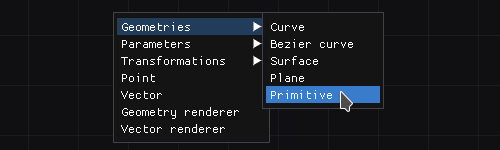
\includegraphics[width=0.75\textwidth]{\fig/ui_1.png}
\item Creare un nodo di \textbf{Geometry Renderer}
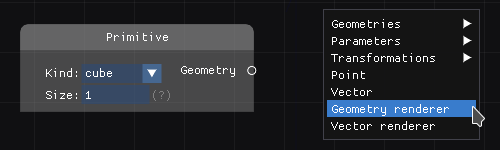
\includegraphics[width=0.75\textwidth]{\fig/ui_2.png}
\end{itemize}
\end{frame}

\begin{frame}
\frametitle{Interfaccia utente}
\centering
\begin{itemize}
\item Collegare i due nodi
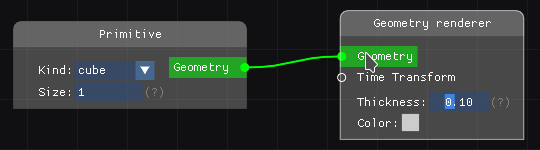
\includegraphics[width=0.75\textwidth]{\fig/ui_3.png}
\item Dalla barra dei pulsanti, clickare su \textbf{Genera Scena}
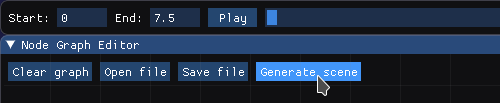
\includegraphics[width=0.75\textwidth]{\fig/ui_4.png}
\end{itemize}
\vspace{0.5cm}
Per zoomare \textbf{nell'editor} tenere premuto \texttt{ctrl} e usare la rotella del mouse.
Per resettare il livello di zoom clickare usando la rotella.
\end{frame}

\section{Trasformazioni}
\begin{frame}
\frametitle{Nota sulle trasformazioni}
Nelle prossime slide seguir\`a l'elenco delle trasformazioni usate
nell'intero corso, la maggior parte di queste non saranno usate in questa esercitazione.
\end{frame}

\begin{frame}
\frametitle{Rotazioni: Asse x}
\begin{equation}
R_x(\theta) = 
\begin{bmatrix}
1 & 0 & 0 \\
0 & \mbox{cos}(\theta) & - \mbox{sen}(\theta)\\
0 & \mbox{sen}(\theta) & \mbox{cos}(\theta)
\end{bmatrix}
\end{equation}
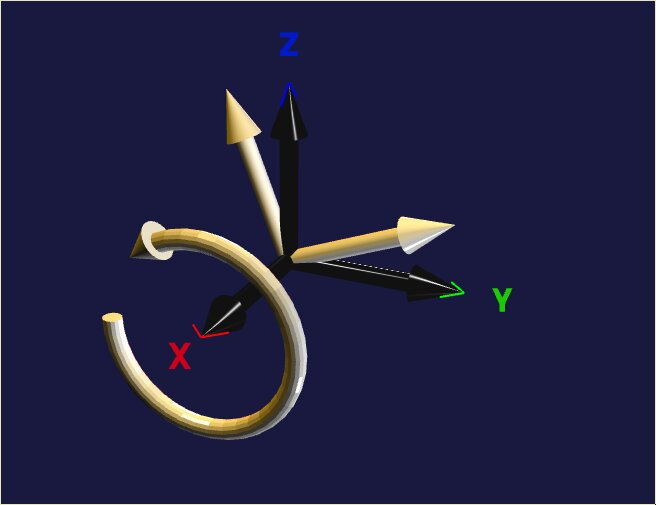
\includegraphics[width=0.6\textwidth]{\fig/rot_x.jpeg}
\end{frame}
\begin{frame}
\frametitle{Rotazioni: Asse y}
\begin{equation}
R_y(\theta) = 
\begin{bmatrix}
\mbox{cos}(\theta) & 0 & \mbox{sen}(\theta)\\
0 & 1 & 0 \\
-\mbox{sen}(\theta)& 0 & \mbox{cos}(\theta)
\end{bmatrix}
\end{equation}
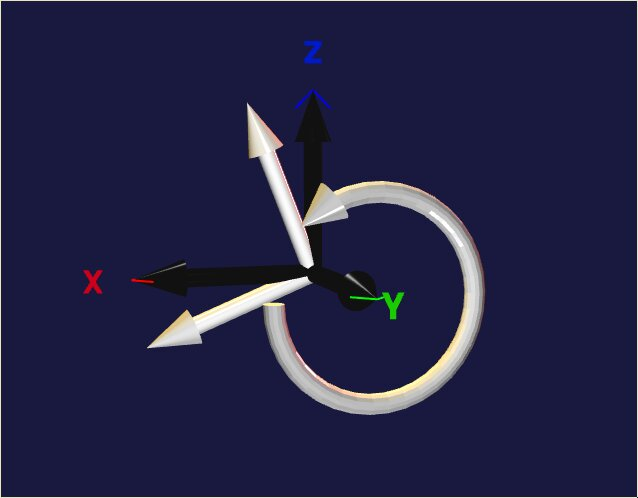
\includegraphics[width=0.6\textwidth]{\fig/rot_y.jpeg}
\end{frame}
\begin{frame}
\frametitle{Rotazioni: Asse z}
\begin{equation}
R_z(\theta) = 
\begin{bmatrix}
\mbox{cos}(\theta) & - \mbox{sen}(\theta) & 0\\
\mbox{sen}(\theta) & \mbox{cos}(\theta)   & 0\\ 
0 & 0 & 1 
\end{bmatrix}
\end{equation}
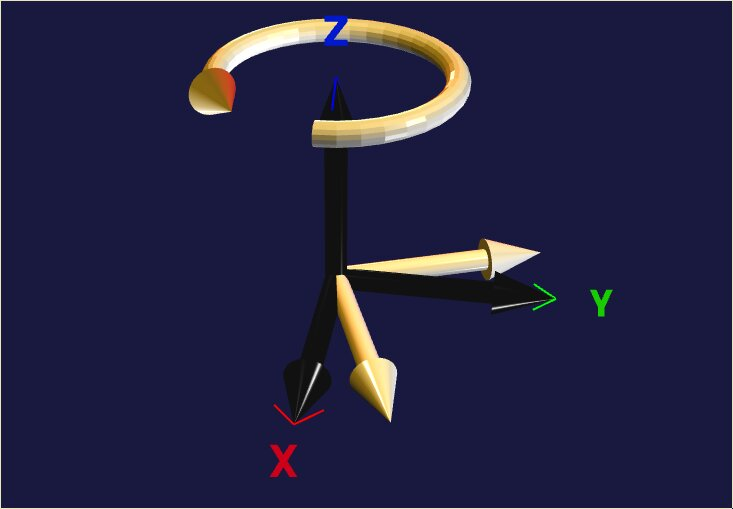
\includegraphics[width=0.6\textwidth]{\fig/rot_z.jpeg}
\end{frame}
%
\begin{frame}
\frametitle{Tagli}
\begin{columns}
\begin{column}{0.48\textwidth}
Taglio in direzione x sulle facce con normale y:
\begin{equation}
T_{xy}=\begin{bmatrix}
    1 & k_x & 0\\
    0 & 1   & 0\\
    0 & 0   & 1
    \end{bmatrix}
\end{equation}
\end{column}
\begin{column}{0.48\textwidth}
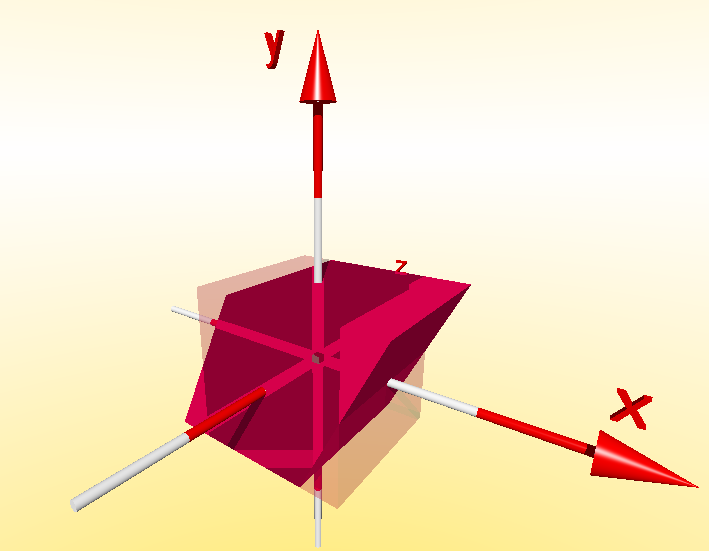
\includegraphics[width=0.8\textwidth]{\fig/cut_tx.png}
\end{column}
\end{columns}
%
\begin{columns}
\begin{column}{0.48\textwidth}
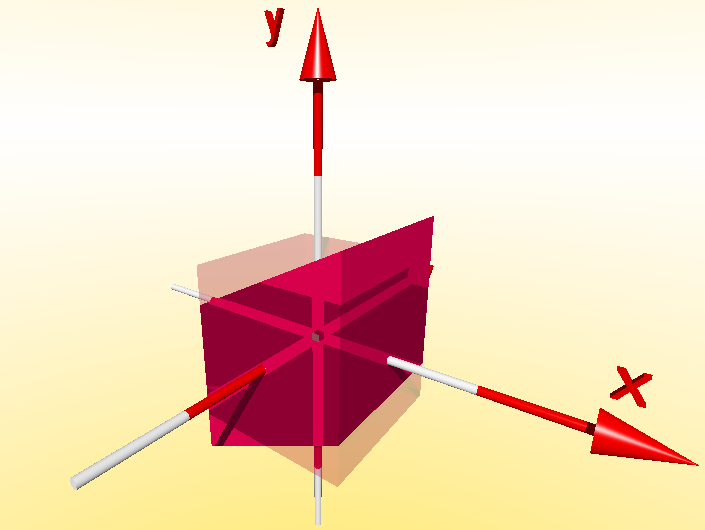
\includegraphics[width=0.8\textwidth]{\fig/cut_ty.png}
\end{column}
\begin{column}{0.48\textwidth}
Taglio in direzione y sulle facce con normale x:
\begin{equation}
T_{yx}=\begin{bmatrix}
    1   & 0 & 0\\
    k_y & 1 & 0\\
    0   & 0 & 1
    \end{bmatrix}
\end{equation}
\end{column}
\end{columns}
\end{frame}
%
\begin{frame}
\frametitle{Tagli[2]}
\begin{columns}
\begin{column}{0.48\textwidth}
Taglio in direzione z sulle facce con normale x:
\begin{equation}
T_{zx}=\begin{bmatrix}
    1 & 0 & 0\\
    0 & 1 & 0\\
    k_z & 0 & 1
    \end{bmatrix}
\end{equation}
\end{column}
\begin{column}{0.48\textwidth}
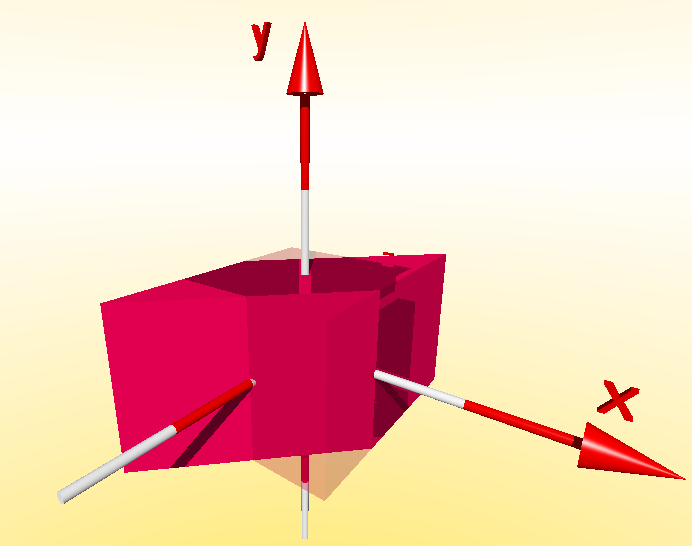
\includegraphics[width=0.8\textwidth]{\fig/cut_tz-x.png}
\end{column}
\end{columns}
%
%\begin{block}{}
\begin{columns}
\begin{column}{0.48\textwidth}
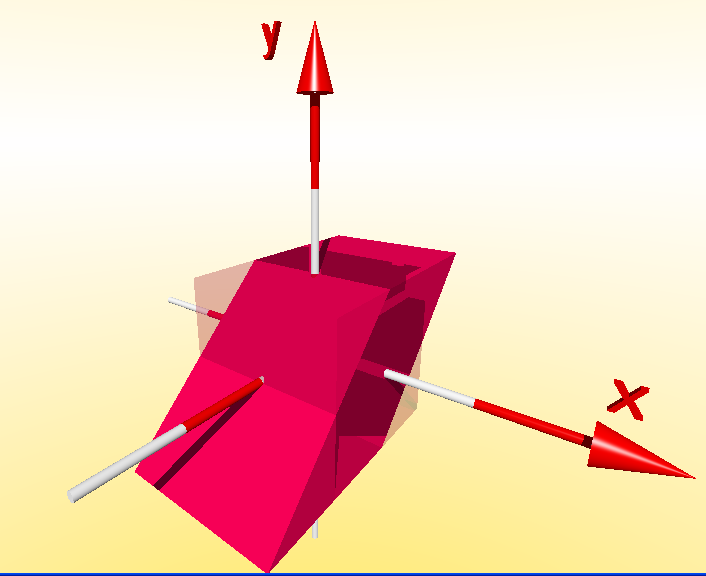
\includegraphics[width=0.8\textwidth]{\fig/cut_tz-y.png}
\end{column}
\begin{column}{0.48\textwidth}
Taglio in direzione z sulle facce con normale y:
\begin{equation}
T_{zy}=\begin{bmatrix}
    1 & 0 & 0\\
    0 & 1 & 0\\
    0 & k_z & 1
    \end{bmatrix}
\end{equation}
\end{column}
\end{columns}
%\end{block}
\end{frame}
%
\begin{frame}
\frametitle{Scalatura, Riflessione,Proiezione}
\begin{itemize}
\item Scalatura
\begin{equation}
S = \begin{bmatrix}
    S_x & 0 & 0\\
    0 & S_y & 0\\
    0 & 0 & S_z
    \end{bmatrix}
\end{equation}
\item Riflessione
\begin{equation}
F = \begin{bmatrix}
      1 & 0 & 0\\
      0 & 1 & 0\\
      0 & 0 & 1
    \end{bmatrix}
    -2~\begin{bmatrix}
    n_x \\
    n_y \\
    n_z
    \end{bmatrix} 
    ~\begin{bmatrix}
    n_x & n_y & n_z
    \end{bmatrix}
\end{equation}
\item Proiezione
\begin{equation}
 P = \begin{bmatrix}
      1 & 0 & 0\\
      0 & 1 & 0\\
      0 & 0 & 1
    \end{bmatrix}
    -\begin{bmatrix}
    n_x \\
    n_y \\
    n_z
    \end{bmatrix} 
    ~\begin{bmatrix}
    n_x & n_y & n_z
    \end{bmatrix}
\end{equation}
\end{itemize}
\end{frame}
%
\begin{frame}
\frametitle{Coordinate omogenee}
\begin{displaymath}
\begin{bmatrix}
a_{11} & a_{12} & a_{13} & t_1 \\
a_{21} & a_{22} & a_{23} & t_2 \\
a_{31} & a_{32} & a_{33} & t_3 \\
0      &    0   &  0     & 1 
\end{bmatrix}
~\begin{bmatrix}
x \\ y\\ z\\ 1
\end{bmatrix}
=  
\begin{bmatrix}
a_{11}x + a_{12}y + a_{13}z + t_1 \\
a_{21}x + a_{22}y + a_{23}z + t_2 \\
a_{31}x + a_{32}y + a_{33}z + t_3 \\
 1
\end{bmatrix}
\end{displaymath}
\end{frame}



\begin{frame}
\frametitle{Coordinate omogenee}
\frnzplt fa uso di matrici di trasformazione in coordinate omogenee, che sono matrici $4 \times 4$.
    \begin{itemize}
        \item Per l'uso odierno, ci basta sapere che quando scriviamo una matrice di trasformazione $3 \times 3$
            dobbiamo scriverla nel blocco in alto a sinistra, lasciando invariato il resto:
    \end{itemize}
\begin{displaymath}
    T = 
\begin{bmatrix}
a_{11} & a_{12} & a_{13} \\
a_{21} & a_{22} & a_{23} \\
a_{31} & a_{32} & a_{33}
\end{bmatrix}
\Rightarrow
\begin{bmatrix}
a_{11} & a_{12} & a_{13} & 0 \\
a_{21} & a_{22} & a_{23} & 0 \\
a_{31} & a_{32} & a_{33} & 0 \\
0      &    0   &  0     & 1 
\end{bmatrix}
\end{displaymath}
\end{frame}

\section{Esercizi}
\begin{frame}
\frametitle{Esercizio 1: prendere familiarit\`a con \frnzplt}
Il nodo \textbf{Primitive} ci fornisce una piccola libreria di figure geometriche primitive, figure solide gi\`a costruite:
    sfera, cubo, cilindro, ecc...
    \vspace {0.75 cm}
Vediamo un altro esempio di utilizzo:
\begin{itemize}
\item Disegnare un cilindro con asse parallelo a $Z$ ed altezza 1.
\begin{itemize}
\item \textit{Elementi da utilizzare:} \\ \texttt{Geometries}$\rightarrow$ \texttt{Primitives}, \\ \texttt{Geometry Renderer}.
\end{itemize}
    \vspace {0.75 cm}
\item Effettuare uno scaling con $S_x =2$, $S_y=1$, $S_z=0.5$.
\begin{itemize}
\item \textit{Elementi aggiuntivi da utilizzare:} \\ \texttt{Transformations}$\rightarrow$ \texttt{Generic Matrix}, \\ \texttt{Transformations}$\rightarrow$ \texttt{Transform}
\end{itemize}
%\item Traslare l'oggetto ottenuto di un vettore a scelta parallelo ad y.
\end{itemize}
\end{frame}
\begin{frame}
\frametitle{Esercizio 1 - i}
\begin{center}
\begin{tikzpicture}
\node(img1){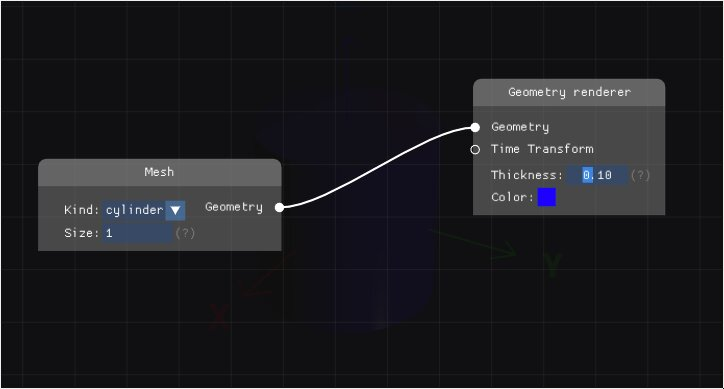
\includegraphics[width=0.7\textwidth]{\fig/l1_cylinder_ex.jpeg}};
\node(img2) at (img1.north west){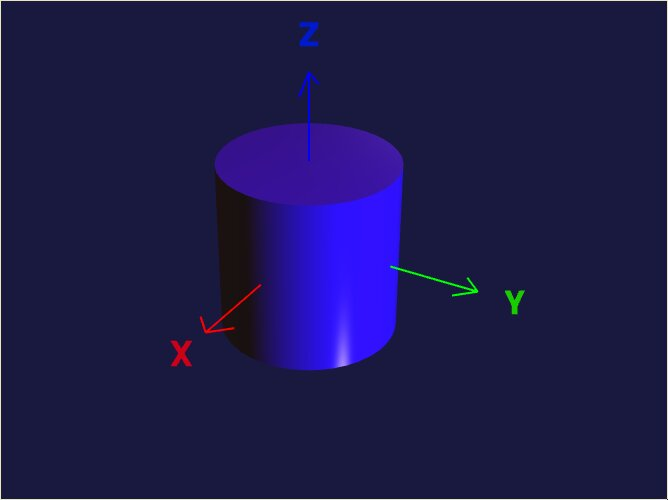
\includegraphics[width=0.4\textwidth]{\fig/l1_cylinder_ex_img.jpeg}};
\end{tikzpicture}
\end{center}
\end{frame}
\begin{frame}
\frametitle{Esercizio 1 - ii}
\begin{center}
\begin{tikzpicture}
\node(img1){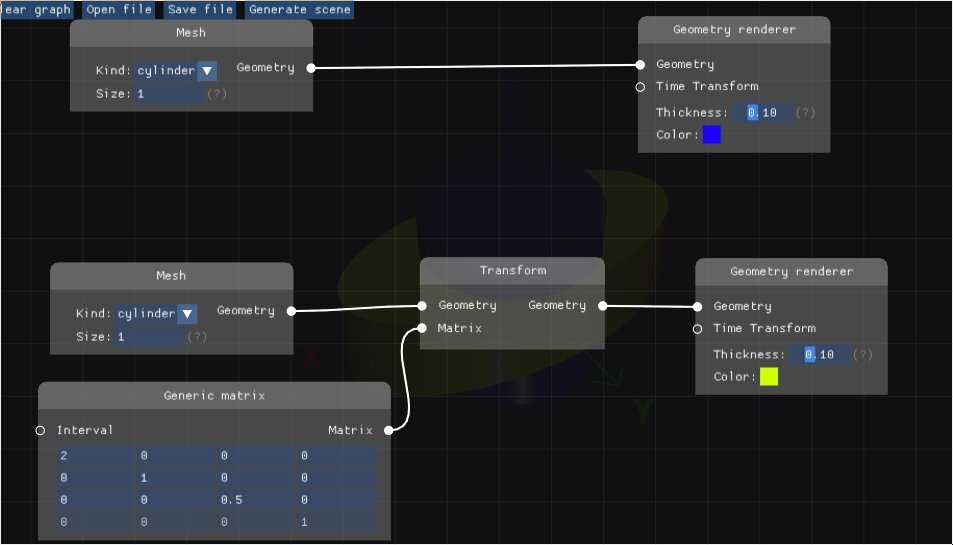
\includegraphics[width=0.7\textwidth]{\fig/l1_cylinder_ex_graph2.jpeg}};
\node(img2) at (img1.north west){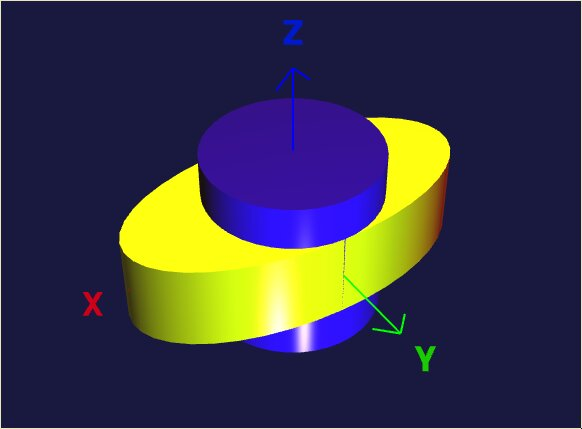
\includegraphics[width=0.4\textwidth]{\fig/l1_cylinder_ex_graph2_img.jpeg}};
\end{tikzpicture}
\end{center}
\end{frame}

\begin{frame}
\frametitle{Esercizio 2: Identificare una trasformazione}
\begin{itemize}
\item Disegnare un  cubo centrato sull'origine, con lati di misura 2 (notare
che nella primitiva \`e possibile fissare un parametro che influenza la
dimensione dell'oggetto).  
\item Applicare al cubo la seguente matrice: 
\begin{displaymath}
A = \begin{bmatrix}
    1 & 0 & 1\\
    0 & 1 & 0\\
    0 & 0 & 1
    \end{bmatrix}
\end{displaymath}
\item Descrivere la deformazione che \`e stata applicata al cubo. Il volume del cubo \`e cambiato?
\end{itemize}
\end{frame}
%
\begin{frame}
\frametitle{Esercizio 2 - i}
\begin{center}
\begin{tikzpicture}
\node(img3){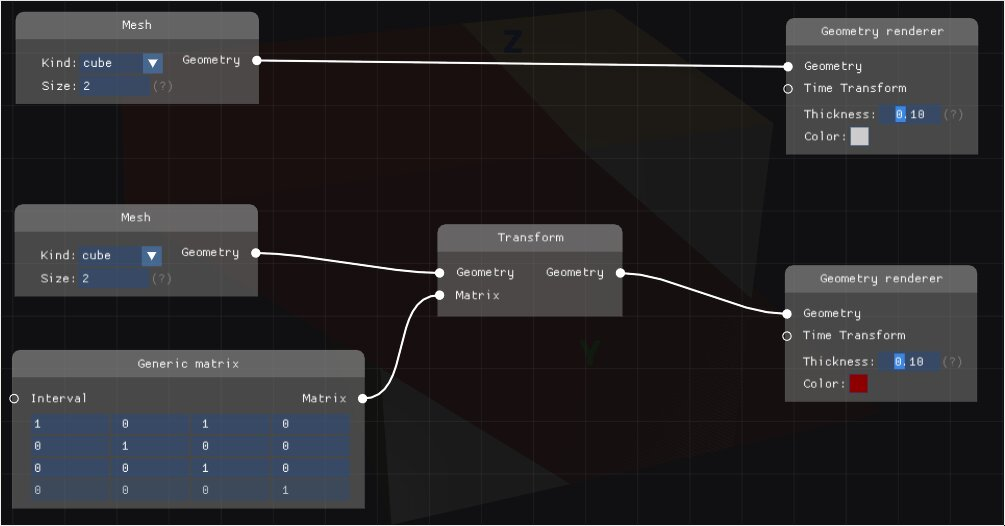
\includegraphics[width=0.7\textwidth]{\fig/l1_es2_graph.jpeg}};
\node(img4) at (img3.south west){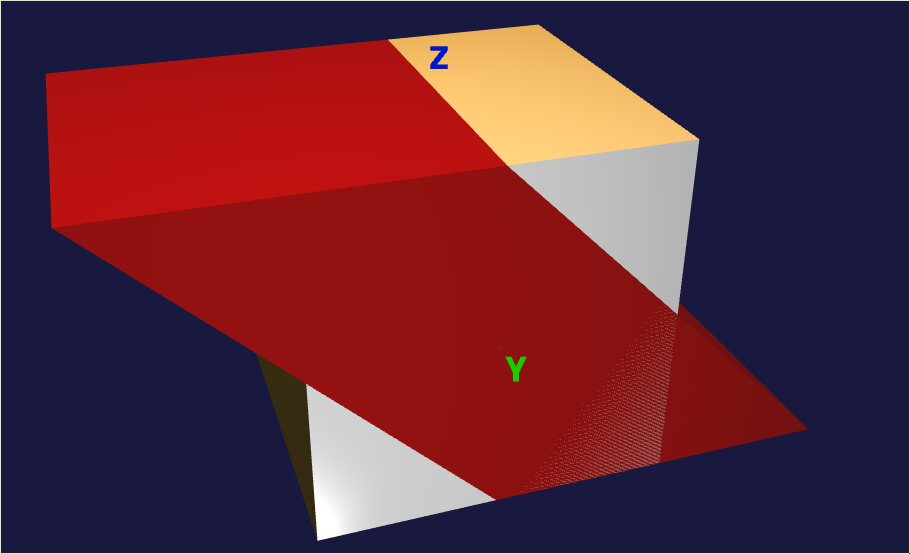
\includegraphics[width=0.4\textwidth]{\fig/l1_es2_img.jpeg}};
\end{tikzpicture}
\end{center}
\end{frame}
% ESEMPIO TRASLAZIONE (SENZA SPIEGAZIONE ) CON TRASFORMAZIONE NEL TEMPO
\begin{frame}
\frametitle{Esercizio 3: Trasformazioni tempo dipendenti}
    \vspace{-0.5cm}
\begin{itemize}
\item Partiamo nuovamente dal cubo dell'es. 2, questa volta applichiamo una trasformazione nel tempo del tipo:
\begin{displaymath}
A = \begin{bmatrix}
    1 & 0 & t \\
    0 & 1 & 0 \\
    0 & 0 & 1
    \end{bmatrix}
\end{displaymath}
\item Utilizzare l'elemento \texttt{Transformations} $\rightarrow$ \texttt{Time Transform}
    \textit{Attenzione: in questa matrice \`e obbligatorio usare la lettera t} \\
        \begin{center}
    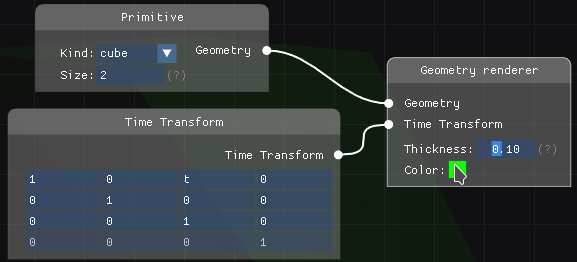
\includegraphics[width=0.6\textwidth]{\fig/l1_es3_modified.png}
        \end{center}
\item Generare la scena e fare click sul tasto \textbf{Play} dalla Top Bar
\end{itemize}
\end{frame}
%%%
%%% l'esercizio numero 4 è stato rifatto da zero visto che non sono ancora state introdotte le trasformazioni necessarie
\begin{frame}
\frametitle {Esercizio 4 - Rotazioni e traslazioni}
Per applicare una trasformazione di rotazione o traslazione abbiamo due alternative:
\begin{itemize}
    \item Scrivere gli elementi nella matrice generica
\end{itemize}
    \begin{center}
    oppure
    \end{center}
\begin{itemize}
\item Usare due nodi contenenti le trasformazioni ``preconfezionate'' (utili per fare test o esperimenti pi\`u velocemente)
\end{itemize}
    \vspace{0.5 cm}
Andiamo a vedere come usare i nodi \texttt{Translation Matrix} e \texttt{Rotation Matrix}
\end{frame}


\begin{frame}
\frametitle {Esercizio 4 - Rotazioni e traslazioni}
\begin{itemize}
    \item Creare un oggetto di tipo `dado' (`\textit{dice}') utilizzando il comando \texttt{Primitive}, con fattore di scala 0.5.
\item Traslare il centro dell'oggetto in $\langle 2,1,0\rangle$  (combinando gli elementi \texttt{Transformations} $\rightarrow$ \texttt{Translation Matrix} e \texttt{Vector}).  
\item Ruotare di 180 gradi il dado traslato intorno all'asse $Z$ (usando l'elemento \texttt{Transformations} $\rightarrow$ \texttt{Rotation Matrix}).  
\item Rappresentare i tre oggetti (iniziale, traslato, traslato e ruotato).
\end{itemize}
\end{frame}

\begin{frame}
\frametitle{Esercizio 4 - i - Dado traslato}
\begin{center}
\begin{tikzpicture}
\node(img1){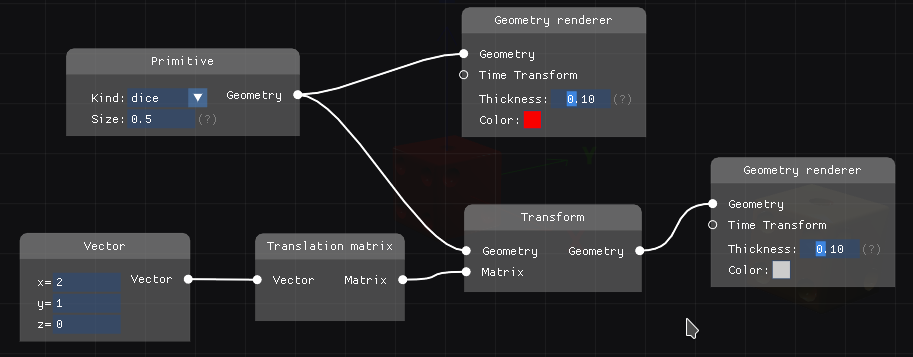
\includegraphics[width=\textwidth]{\fig/l1_es4_translation.png}};
%\node(img2) at (img1.north west){\includegraphics[width=0.4\textwidth]{\fig/snapcode_3-3.png}};
\end{tikzpicture}
\end{center}
\end{frame}
\begin{frame}
\frametitle{Esercizio 4 - ii - Trasformazioni in cascata}
\begin{center}
\begin{tikzpicture}
\node(img1){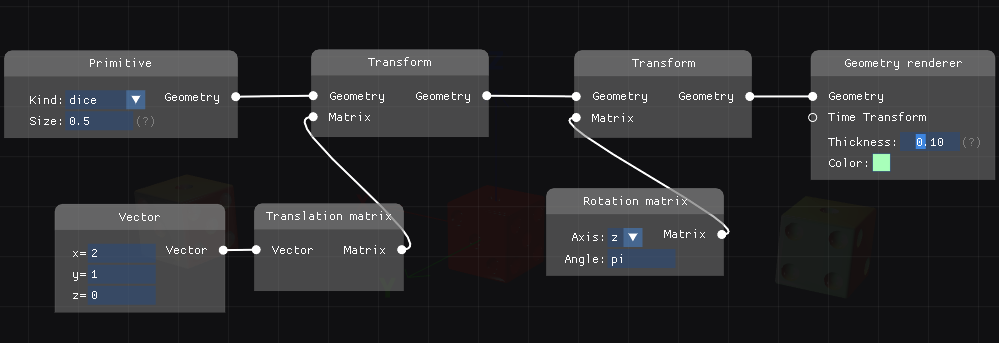
\includegraphics[width=\textwidth]{\fig/l1_es4_chained.png}};
%\node(img2) at (img1.north west){\includegraphics[width=0.4\textwidth]{\fig/snapcode_3-3.png}};
\end{tikzpicture}
\end{center}
\end{frame}
\begin{frame}
\frametitle{Esercizio 4 - iii - Risultato}
\begin{center}
\begin{tikzpicture}
\node(img1){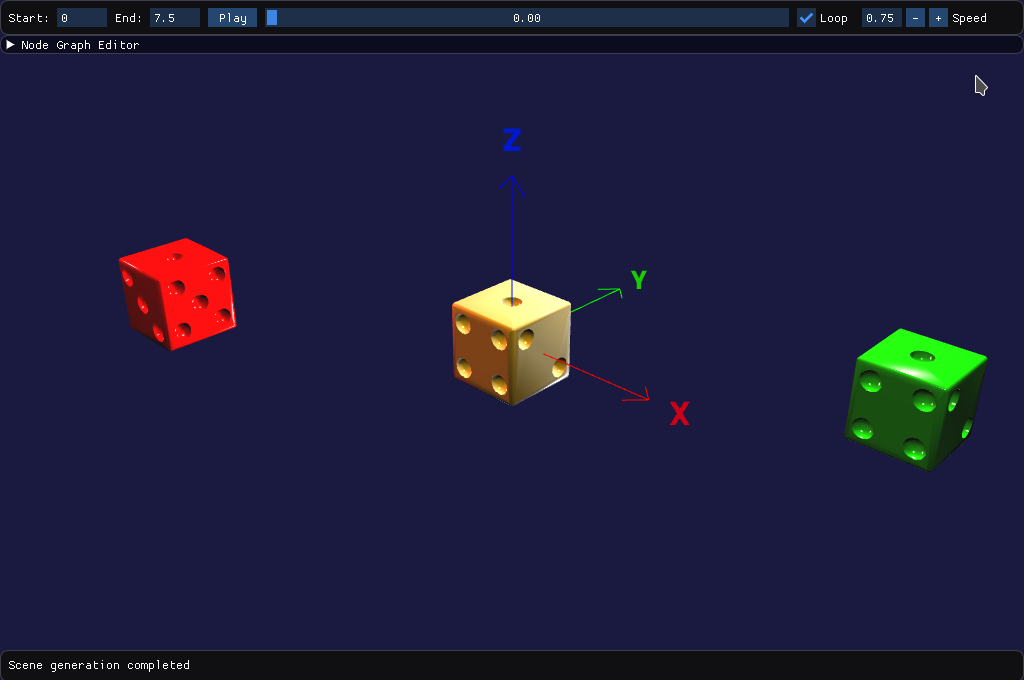
\includegraphics[width=\textwidth]{\fig/l1_es4_result.png}};
%\node(img2) at (img1.north west){\includegraphics[width=0.4\textwidth]{\fig/snapcode_3-3.png}};
\end{tikzpicture}
\end{center}
\end{frame}

\begin{frame}
\frametitle{Esercizio 4 - iv - Considerazioni finali}
\begin{itemize}
\item \`E possibile verificare che il dado sia stato ruotato correttamente controllando come sono orientate le facce.
\item Se vogliamo animare la rotazione usando la \texttt{Time Transform}, sar\`a necessario scrivere la matrice ``a mano''
    (non \`e possibile usare il nodo Rotation Matrix).
\item Cambiando l'ordine delle trasformazioni (applicando la rotazione \textit{prima} della traslazione),
    il risultato finale \`e lo stesso o cambia?
\end{itemize}
\end{frame}

\begin{frame}
\frametitle{Per Casa: Proiezioni ortogonali}
\begin{columns}
\begin{column}{0.32\textwidth}
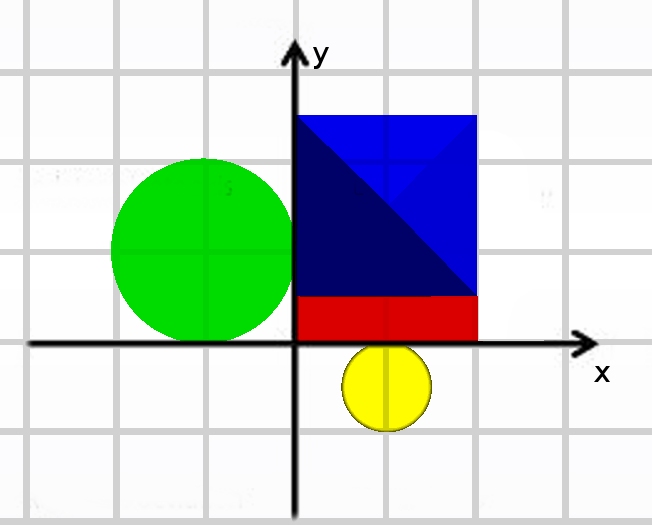
\includegraphics[width=\textwidth]{\fig/proj1.png}
\end{column}
\begin{column}{0.32\textwidth}
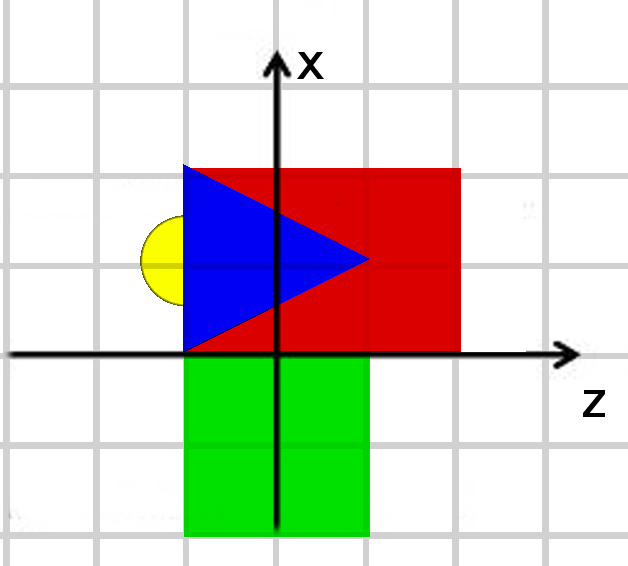
\includegraphics[width=\textwidth]{\fig/proj2.png}
\end{column}
\begin{column}{0.32\textwidth}
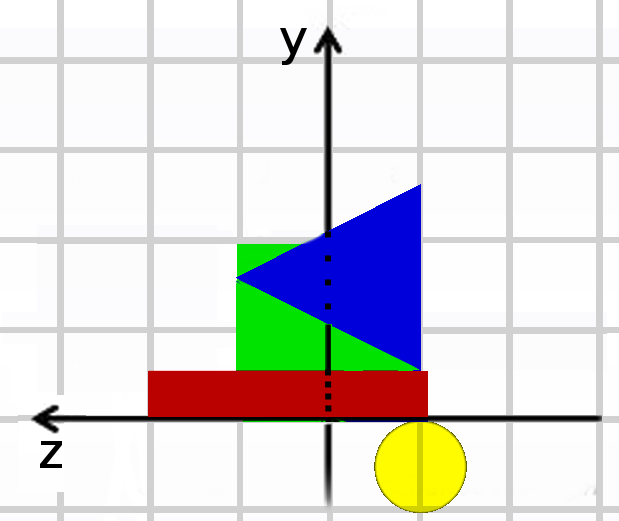
\includegraphics[width=\textwidth]{\fig/proj3.png}
\end{column}
\end{columns}
\vspace{20pt}
Creare un'organizzazione di oggetti le cui proiezioni sui piani cartesiani riproducono le figure sovrastanti.
\end{frame}

\end{document}

